\documentclass[titlepage,12pt]{article}
\usepackage[romanian]{babel}
%\usepackage{mathptmx}
%\usepackage[T1]{fontenc}
%\usepackage[utf8]{inputenc}
\usepackage{fontspec}
\setmainfont{Times New Roman}
\usepackage[backend=biber]{biblatex}
\usepackage{listings, listings-rust, docker}
\usepackage{xcolor}
\usepackage{multicol}

\lstset{
    basicstyle=\fontsize{10}{12}\selectfont\ttfamily\usefont{T1}{zi4}{m}{n}
    keywordstyle=\color{blue}\bfseries, % Keywords in blue and bold
    commentstyle=\color{green}, % Comments in green
    stringstyle=\color{red}, % Strings in red
    backgroundcolor=\color{lightgray}, % Light gray background
    frame=single, % Frame around the code
    numbers=left, % Line numbers on the left
    stepnumber=1, % Step between line numbers
    numberstyle=\tiny\color{gray}, % Style for line numbers
}
%\def\ttdefault{blg}
\addbibresource{doc.bib}
\usepackage[
top=2cm,
bottom=2cm,
left=2cm,
right=2cm]{geometry}
\usepackage{setspace}
\usepackage{indentfirst}
\usepackage{graphicx}
\usepackage{caption}
\usepackage{longtable}
\usepackage{acronym}
\usepackage{float}
\renewcommand{\baselinestretch}{1.0}
%\renewcommand{\ttfamily}{\fontsize{10pt}{12pt}\selectfont}
% use [Ref n] instead of [n]
\DeclareFieldFormat{labelnumber}{Ref~\thefield{labelnumber}}
%spacing 1
%Text normal: 12 size, proportional serif
%Cod sursa: fixed width, 8..12 size, fixed width

\begin{document}
% Title
\title{Licenta}
\author{Popescu Ionut-Alexandru}
\date{\today}

\maketitle
\renewcommand{\contentsname}{Cuprins}
\renewcommand{\listfigurename}{Lista figurilor} 
\renewcommand{\listtablename}{Lista tabelelor}
\renewcommand{\figurename}{Figura}
\renewcommand{\tablename}{Tabela}
% Table of Contents
\tableofcontents
\clearpage  
\listoffigures
\clearpage
\listoftables
\clearpage
\section*{Lista acronimelor} % Use \section* to avoid it being numbered
\begin{acronym}  
    \acro {Z80}       {Microcontroler Zilog Z80}
    \acro {I8080}     {Intel 8080}
    \acro {IO}        {Input/Output}
    \acro {ROM}       {Read Only Memory}
    \acro {RAM}       {Random Access Memory}
    \acro {Rust}      {Limbajul de programare Rust}
    \acro {WASM}      {Web Assembly}
    \acro {DARPA}     {Defense Advanced Research Projects Agency}
    \end{acronym}
\clearpage
% Sections

\section{Introducere}
Acest proiect reprezinta un emulator complet functional pentru un \ac {Z80}, implementat complet in \ac {Rust}.
Emulatorul este conceput sa functioneze ca o librarie flexibila ce poate fi inclusa cu usurinta in alte proiecte scrise Rust. Acest lucru permite utilizatorilor sa il adapteze la propriile necesitati.

\ac {Z80} este un procesor pe 8 biti, produs din 1976 de catre firma Zilog. Desi acest procesor are magistrala de adrese de 16 biti, magistrala de adrese este de 8 biti.
Desi registrii procesorului functioneaza pe 8 biti, acesta poate face operatiuni pe valori de 16biti prin folosirea registrilor combinati(BC,DE,HL).
Z80 are are un set de 158 tipuri de instructioni considerate oficiale, dar exista si altele care nu au fost documentate oficial de Zilog. Instructiunile pot face o multime de operatiuni cum ar fi: transfer de date, interschimbare, operatiuni aritmetice/logice, rotiri/shiftari, instructiuni la nivel de bit si comunicare cu porturile I/O.

Impreuna cu libraria ce se ocupa strict cu partea de emulate, proiectul contine si o aplicatie web bazata pe aceasta librarie.
Aceasta aplicatie web este de asemenea scrisa in Rust, apoi compilata in \ac {WASM}. Deoarece \ac {WASM} este mai preformant decat JavaScript, aceasta compilare din Rust va aduce un bonus de performanta, un lucru necesar pentru o emulare cat mai fluida.
Principalul avantaj compilarii programului in \ac {WASM} a fost avantajul dat de faptul ca acest lucru ii va permite sa ruleze din orice browser web modern.
Aplicatia web este de tipul server-client insa ofera si capacitatea de a rula standalone, putand fi utilizate si fara server in modul offline.

Motivatia principala a acestui proiect a fost lipsa unui astfel de emulator, acestea fiind putine, reprezentan uneori dificultati la instalare sau unele fiind chiar incomplete.
Acest proiect isi propune sa ofere o solutie completa, accesibila si usor de folosit si de integrat in alte proiecte. Un alt scop de asemene al acestei lucrari, poate fi unul educativ, oferind un mediu usor de dezvoltare si testare.

Emulatorul ar trebui sa faciliteze utilizatorului un mod cat mai usor de a dezvolta aplicatii pe platforma Z80.
Libraria permite direct scrierea de cod in Assembly iar apoi rularea acestuia in cadrul emulatorului. Acest lucru va permite utilizatorului sa testeze si sa depaneze aplicatia fara a avea nevoie de un hardware real.
Pe langa faptul ca utilizatorul poate sa puna pauza executiei in orice moment si sa vizualizeze registrii, este de asemenea posibila si modificarea acestora.
Acest control fin asupra executiei aplcatiei, ar trebui sa confere un avantaj in dezvoltarea aplicatiilor, permitand o monitorizare cat mai buna asupra cursului executiei.

Pentru o simulare cat mai corecta si apropiata de un Zilog Z80 adevarat, toate instructiunile acestuia au fost implementate. 
Executarea instructiunilor se face cat mai realist si tinand cont de factori cum ar fi: lungimea instructiunii, ciclurile acesteia si a vitezei de ceas(clock) aleasa.
Memoria emulatorului de asemenea este complet configurabila de catre utilizator, acesta putand fi configurata ca fiind \ac {ROM}/\ac {RAM} sau chiar nealocata.


\section{Stadiul actual}
This is the introduction.

\section{Fundamentare teoretica}
This is the main section.

\section{Cercetare}
Pentru a putea realiza acest proiect, a fost necesara o cercetare amanuntita a din capitolele de mai jos.
Prin aceasta cercetare s-a putut pune la punct o arhitectura structurala a proiectului, pregatita de faza de implementare.

\subsection{\ac {Z80}}
Procesorul Z80 (Fig~\ref{fig:z80}) este un procesor pe 8 biti, produs de Zilog in 1976. Acesta este unul dintre cele mai populare procesoare din istorie, fiind utilizat in multe aplicatii, de la calculatoare personale la console de jocuri.
\ac {Z80} este un procesor CISC, acesta avand un set de 158 de instructiuni oficiale, dar exista si altele care nu au fost documentate oficial de Zilog.

\begin{figure}[H]
    \centering
    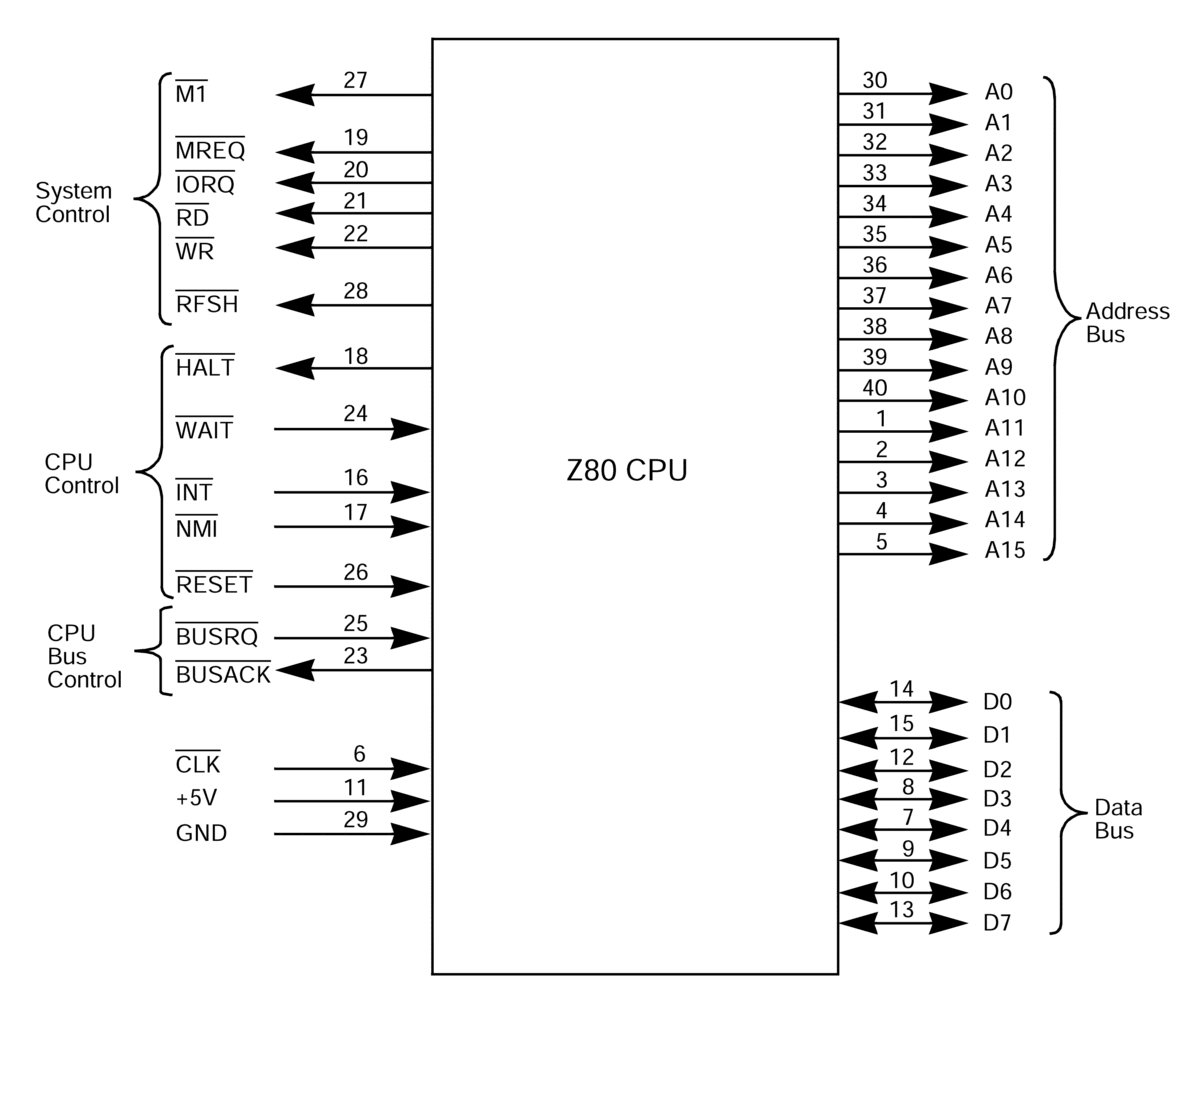
\includegraphics[width=0.5\textwidth]{images/z80.jpg}
    \caption{Microprocesor Z80.}
    \label{fig:z80}
\end{figure}

\subsubsection{Registrii}
\cite{ref:z80instructions}Procesorul are 10 registrii pe 8 biti,8 din care sunt pentru uz general, si 4 registrii pe 16 biti.
Rolul registrilor:
\begin{itemize}
    \item A,B,C,D,E,H,L sunt registrii de uz general pe 8 biti.
    \item F este un registru de flaguri.
    \item PC este un registru pe 16 biti care contine adresa instructiunii curente.
    \item SP este un registru pe 16 biti care contine adresa stivei.
    \item IX si IY sunt registrii pe 16 biti folositi pentru indexare.
    \item I este un registru pe 8 biti folosit pentru intreruperi.
    \item R este un registru pe 8 biti folosit pentru temporizare.
    \par \hspace{1em} \textit{Acesta este incrementat cu 1 la fiecare instructiune executata.}
    \item AF, BC, DE si HL sunt registrii de uz general pe 16 biti, fiecare fiind format de 2 registrii pe 8 biti.
\end{itemize}
Structura acestora se poate vedea si in Figura \ref{fig:z80registers}.
\begin{figure}[H]
    \centering
    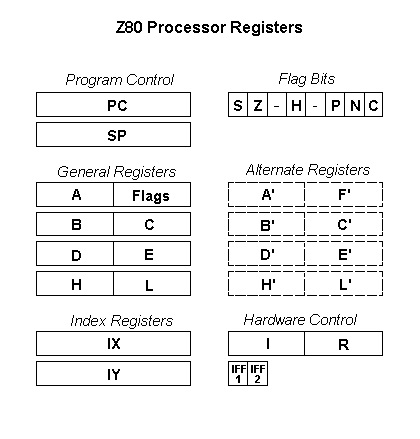
\includegraphics[width=0.5\textwidth]{images/z80registers.jpg}
    \caption{Structura registrii Z80. \cite{ref:z80registers}}
    \label{fig:z80registers}
\end{figure}

Registrul F este un registru de flaguri, acesta contine informatii despre rezultatele operatiilor aritmetice si logice.
Structura acestuia se poate vedea si in Tabela \ref{tab:z80flags}.
\begin{table}[h]
    \centering
    \begin{tabular}{|c|c|c|c|c|c|c|c|c|}
    \hline
    \textbf{Bit} & 7 & 6 & 5 & 4 & 3 & 2 & 1 & 0 \\
    \hline
    \textbf{Flag} & S & Z & F5 & H & F3 & P/V & N & C \\
    \hline
    \end{tabular}
    \caption{Z80 Flags}
    \label{tab:z80flags}
\end{table}

\subsubsection{Memorie}

Desi microprocesorul are magistrala de date pe 8 biti, acesta foloseste 16 biti pentru adresare. Datorita acestui lucru capacitatea maxima de memorie este de \(2^{16}=65536\) octeti. Aceasta zona de memorie de 64K poate fi separata intre \ac {ROM} si \ac {RAM} in functie de implementare.

Unele periferice in aceste sisteme sunt legate direct la memorie, acest lucru permitand microprocesorului sa comunice cu dispozitive externe prin simple scrieri si citiri din memorie.

Un exemplu de astfel de dispozitiv ar putea fi un ecran extern, fiecare pixel de pe acesta fiind reprezentat de o locatie in memorie, valoarea din aceasta specificand culoarea pixelului.

\subsubsection{Instructiuni}

Modelul oficial al \ac {Z80} contine 158 de instructiuni. Luand in considerare fiecare variatie a acestora, numarul total de instructiuni este de 696.
Instructiunile sunt impartite in 8 categorii principale:
\begin{itemize}
    \item Load si Exchange
    \item Transfer bloc de date si cautare
    \item Aritmetice si logice
    \item Rotiri/Shiftari
    \item Instructiuni la nivel de bit
    \item Jump/Call/Return
    \item \ac {IO}
    \item Control
\end{itemize}

Instructiunile de tip Load sunt cele care copiaza datele intern intre registrii sau intre registrii si memoria externa.
Toate aceste instructiuni specifica o locatie sursa de unde sa fie copiata valoarea si o destinatie unde sa fie copiata aceasta.
Locatia sursa nu este afectata de aceste instructiuni, aceasta fiind doar citita.
Exemple de asfel de instructiuni sunt cele care copiaza valoarea dintr-un registru in altul "LD A,B" sau cele care copiaza valoarea dintr-o locatie de memorie in registru "LD A,(HL)".

Instructiunile de tip exchange sunt cele care interschimba valorile dintre registrii.\\

Un set unic de instructiuni de transfer al blocurilor de date sunt include in \ac {Z80}.
Cu o singura instruciune, un bloc din memorie de orice marime poate fi mutat in orice alta locatie din memorie.
Aceste instructiuni sunt foarte folositoare in procesarea sirurilor de caractere.
Cu o singura instructiuni, un bloc intreg de de memorie de orice marime poate fi cautat dupa un anumit byte.
Cand valoarea este gasita sau se ajunge la sfarsitul blocului, instructiunea se opreste automat.
Instructiunile de acest tip permit intreruperile sa fie procesate in timpul executiei lor, astfel incat procesorul nu este blocat pentru perioade lungi de timp.\\

Instructiunile aritmetice si logice opereaza pe datele stocate in acumulator si alti registrii sau valori din memorie.
Rezultatul operatiei este stocat in acumulator.
De asemenea registrul de flaguri este actualizat in functie de rezultatul operatiei.\\

Rotate si Shift sunt grupuri de instructiuni care permit registrilor cat si valorilor din memorie sa fie rotite sau shiftate la stanga sau dreapta, cu sau fara carry.\\

Operatiunile la nivel de bit permit oricarui bit din acumulator, alt registru sau o locatie din memorie sa fie setat, resetat sau testat.\\

Jump, Call si Return sunt tipuri de instructiuni care transfera executia programului la o alta locatie din memorie.
Aceste instructiuni folosesc mai multe metode diferite de a transfera controlul programului.
Instructiunea Reset este un tip special de Call care permite saltul la doar 8 locatii diferite din memorie.
Alte instructiuni permit incarcarea Program Counter (PC) direct cu o valoare din memorie specificata de HL, IX sau IY.
Aceste instructiuni permit un nivel de control foarte inalt asupra executiei programului.\\

Instructiunile de \ac {IO} permit un spectru larg de transferuri de date intre microprocesor si dispozitivele externe.
O instructiune de acest tip foloseste ca port in transfer al doilea byte al instructiunii.
Alta instructiune permite portului sa fie specificat de registrul C.
Un avantaj mare in a folosi portul C, este ca permite unei functii sa fie refolosita pentru orice port.
Acest lucru nu ar fi posibil daca portul ar fi specificat de al doilea byte al instructiunii.
O buna caracteristica a acestor instructiuni este ca modifica automat flagurile in functie de rezultatul operatiei.
Din acest motiv nu este necesar sa se faca verificari suplimentare pentru a testa rezultatul operatiei. Exemplu: flagul de semn este setat daca rezultatul operatiei este negativ.\\

\ac {Z80} include instructiuni care sunt capabile sa mute blocuri intregi de date (pana la 256 byte) automata intre orice port \ac {IO} si memorie
Impreuna cu setul dual de registrii cu scop general, aceste instructiuni faciliteaza transferuri rapide de rate cu dispozitivele externe.\\

Instructiunile de control sunt instructiuni care controleaza mici aspecte ale microprocesorului.
Unele instructiuni de acest tip sunt cele care activeaza sau dezactiveaza intreruperile, sau cele care controleaza modul de raspuns la intreruperi.

\subsection{Emulator}
Un emulator reprezinta o metoda hardware sau software de a imita un alt tip de sistem de calcul, cum ar fi un procesor, consola sau chiar un intreg calculator.

In cazul acestui lucrari s-a ales un emulator software, acesta fiind mult mai accesibil.

Principala aplicatie a unui emulator este de a rula un program scris pentru o anumita arhitectura pe una complet diferita.

Acest lucru ajuta in mentenanta pe termen lung permitand inlocuirea componentei hardware vechi cu una mai noua fara a necesita software nou.

In cazul curent, deoarece \ac {Z80} este destul de vechi si procurarea acestuia a devenit o problema, in cazul in care microcontrolerul necesita inlocuirea, acesta va putea fi inlocuit cu un Raspberry Pi (sau o alternativa) ruland un emulator.

Pentru realizarea proiectului, emulatorul este necesar sa contina memoria, registrii, si logica necesara pentru decodarea si executarea instructiunilor.

Emularea se va face cat mai apropiat de un Z80 real, acest lucru fiind necesar pentru a asigura ca aplicatiile scrise pentru Z80 vor rula corect.
Pentru asigurarea calitatii si corectitudinii, toate instructiunile Z80 vor fi implementate, acestea fiind testate cu ajutorul unor teste unitare.

Emularea va functiona la nivel de instructiune, acest lucru permitand o monitorizare cat mai buna a executiei programului.
Utilizatorul va avea in fiecare moment control asupra executiei programului, acesta putand pune pauza executiei, modifica registrii sau vizualiza memoria.
Aceste facilitati ar trebui sa ofere un avantaj enorm in depanarea aplicatiilor scrise pentru Z80.
Un asemenea debugger ii va permite programatorului sa vada exact ce se intampla in fiecare moment al executiei programului.

Deoarece se vrea un nivel cat mai inalt de control, memoria emulatorului de asemenea va putea fi configurata.
Zone intregi de memori pot fi alocate ca fiind \ac {ROM} sau \ac {RAM}, sau chiar nealocate.
Deoarece codul va rula in emulator, in cazul accesarii unei zone de memorie nealocate, acest lucru va fi detectat si va fi notifica utilizatorul.

Pentru a simula dispozitivele externe, emulatorul va avea si un sistem de porturi \ac {IO}.
Porturile \ac {IO} in cazul emulatorului, vor fi legate la niste dispozitive virtuale care vor simula dispozitivele reale.
Aceste dispozitive virtuale vor fi configurabile de catre utilizator, acesta putand alege ce dispozitive sa fie simulate si ce porturi sa fie folosite.
Exemplu: Emulatorul va putea simula accesul la un ecran, tastatura sau chiar un dispozitiv de stocare.

O alta caracteristica pe care o va avea emulatorul este cea de extensibilitate.
Emulatorul va fi scris ca o librarie, acesta putand fi inclus in orice alt proiect scris in Rust.
Acest lucru va permite utilizatoriilor sa isi creeze propriile dispozitive compatibile cu emulatorul.
Exemplu: Un utilizator ar putea sa creeze un dispozitiv care sa simuleze un ecran cu o rezolutie mai mare


%\begin{multicols}{2}

%\begin{lstlisting}[language=C++]
%#include <iostream>
%using namespace std;
%
%int main() {
%    cout << "Hello, C++!" << endl;
%    return 0;
%}
%\end{lstlisting}
%\end{multicols}

\subsection{Decizie limbaj de programare}

In procesul de alegere a limbajului de programare, s-au luat in considerare mai multe aspecte, cum ar fi:
performanta, documentatie si securitate.

Performanta este un aspect important, deoarece emulatorul va trebui sa ruleze cat mai fluid si cat mai apropiat de un Z80 real.
Un emulator eficient putand fi capabil sa ruleze in functie de nevoie chiar mai rapid.

Din aceasta cauza a fost preferat un limbaj compilat ce permite un control mai fin asupra memoriei si a resurselor.

Limbaje cum ar fi JavaScript si Python desi capabile, ar avea probleme in a mentine nivelul de performanta necesar unui astfel de emulator.

Un limbaj foarte folosit, mai ales pe embedded este C/C++, acesta fiind considerat a fi printre cele mai rapide.

Alt limbaj care a fost luat in considerare a fost Rust, acesta fiind un limbaj modern,
care oferta acelasi nivel de control si performanta ca C/C++, dar cu un sistem de tipuri mai sigur si mai usor de folosit.

Un mare avantaj al \ac {Rust} este sistemul sau de tipuri si de ownership,
acesta putand preveni multe buguri comune din C/C++ cum ar fi race conditions, memory leaks sau dereferentierea unui pointer null.

In \ac {Rust} nu exista pointeri null, acest lucru fiind inlocuit de tipul Option<T>,acesta fiind un enum care poate fi Some(T) sau None.

Datorita nivelului ridicat de securitate adus de Rust,
\ac {DARPA} a lansat proiectul TRACTOR, acest proiect are ca tinta transformarea automata a codului C/C++ in Rust.

Un alt motiv din cauza carui \ac {Rust} a fost ales ca limbaj pentru proiect, este faptul ca acesta poate fi compilat cu usurinta in \ac {WASM},
acest lucru va permite rularea aplicatiei in orice browser web modern.

\subsection{Web}

In ultimii ani, aplicatiile web au devenit din ce in ce mai populare, acestea fiind usor de accesat si de folosit.
Un avantaj major al aplicatiilor web este faptul ca acestea pot rula pe orice dispozitiv care are un browser web.
Datorita avansarii rapide in tehnologie, acum se pot gasi pe piata frigidere si masini de spalat care au un browser web, lucru care ar fi fost greu de crezut acum 20 ani.

Un alt avantaj al aplicatiilor web este faptul ca acestea pot fi rulate fara a fi instalate, acest lucru fiind un avantaj major in cazul unui emulator.
Mare parte din emulatoarele existente necesita instalare, acest lucru fiind un inconvenient pentru utilizatorii care nu doresc sau nu pot sa faca acest lucru.
Deoarece aplicatia este ruleata din browser, utilizatorul nu risca sa descarce un virus, aplicatia web neavand access direct asupra calculatorului.
Un alt avantaj a creari unei aplicatii web este ca emulatorul va fi capabil sa ruleze pe orice arhitectura de procesor sau sistem de operare, atat timp cat acesta are un browser web modern.

Desi aplicatia web va fi capabila sa functioneze in mod standalone, complet offline, aceasta va putea fi integrata si in alte aplicatii web, oferind un nivel de control mai mare asupra acesteia.

In proiectul curent, va fi de asemenea folosit si un server pentru partea de backend. Desi nu este necesar, acesta este folosit pentru a oferi o experienta mai buna utilizatorului.
Anumite actiuni, cum ar fi compilarea codului C in cod Z80, nefiind posibile in browser, acestea fiind procesate de backend si apoi transmise inapoi catre client.

Contrar multor aplicatii web, aceasta nu va folosi javascript, singura parte de javascript fiind cea care incarca aplicatia \ac {WASM} in browser.
\ac {WASM} a fost ales deoarece este mult mai performant decat javascript, acesta fiind capabil sa ruleze cod mult mai rapid. De asemenea, deoarece fisierele ".wasm" sunt in format binar,
nu text precum javascript, acestea sunt mult mai compacte, ocupand mai putin spatiu si facilitand o incarcare mai rapida a aplicatiei.

\ac {Rust} a fost folosit ca limbaj de programare atat pentru frontend cat si pentru backend.
Folosirea aceluiasi limbaj de programare pe ambele parti, va facilita dezvoltarea si mentenanta aplicatiei.

Serializarea si deserializarea datelor reprezinta procesul prin care structuri de date complexe sunt convertite in format text sau binar, pentru a putea fi transmise pe retea sau salvate pe disk.
In cazul aplicatiei web, serializarea si deserializarea datelor este necesara pentru a putea transmite datele de la client la server si invers.
Pentru aceasta, se va folosi formatul JSON, acesta fiind un format des folosit pentru web, si foarte bine suportat de \ac {Rust}.
Datorita librariei de serializare/deserializare Serde, aceasta operatie este foarte usoara si rapida de realizat.
Toate structurile de date fiind serializabile/deserializabile cu modificari minime.
Acest lucru ne face foarte usoara transmiterea de obiecte intre server si client.

Serverul aplicatiei va avea access la randul sau la o baza de date, aceasta oferind functionalitatile extra doar utilizatorilor logati.
Pentru o securitate cat mai buna, parolele nu vor fi salvate direct in baza de date.
In schimb, acestea vor fi criptate folosind algoritmul de hashing argon2.
Aceasta metoda de criptare este una dintre cele mai sigure, aceasta fiind capabila sa reziste unor atacuri brute force chiar si pe cele mai puternice calculatoare.

De asemenea, un sistem de tokenuri va fi folosit pentru a autentifica utilizatorii.
Acest lucru va permite serverului sa stie daca un utilizator este logat sau nu, fara a fi nevoie de a trimite parola la fiecare request.
Un token unic este creat de server la fiegare logare, acesta fiind trimis inapoi si stocate in browser de catre client.
Server apoi la fiecare request va verifica daca tokenul este valid si daca este, va permite accesul la resursele protejate.

\subsection {Docker}

Docker\cite{ref:docker} este o platforma ce permite dezvoltarea, livrarea si rularea aplicatiilor.
Docker ofera posibilitatea de a separa aplicatia de infrastructura, acest lucru permitand rularea acesteia pe orice sistem care are Docker instalat.
Un container Docker este o unitate standard de software care incorporeaza codul aplicatiei, librariile si dependintele acesteia, impreuna cu un mediu de runtime bazat de obicei pe un sistem de operare Linux.
Fiecare container este complet izolat de celelalte, acest lucru permitand rularea mai multor aplicatii pe acelasi sistem fara a interfera intre ele.
Desi fiecare container este izolat, acesta pot fi configurate sa comunice cu alte containere sau cu sistemul gazda, acest lucru permitand crearea de aplicatii complexe.

Desi containerele par similare cu masinile virtuale, acestea sunt mult mai mici, rapide si eficiente.
Un container va rula pe acelasi kernel ca si sistemul gazda, acest lucru facandu-l mult mai eficient decat o masina virtuala.

\begin{figure}[H]
    \centering
    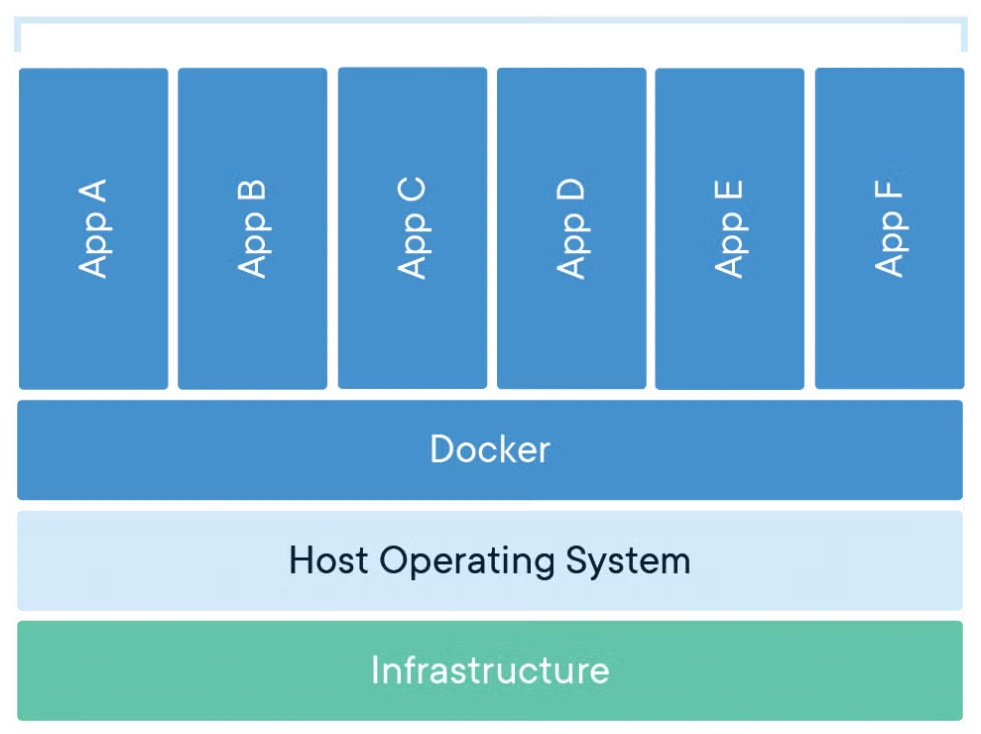
\includegraphics[width=0.7\textwidth]{images/dockerstructure}
    \caption{Structura Docker.}
    \label{fig:containerstructure}
\end{figure}

In cazul aplicatiilor cu trafic mare, Docker ofera posibilitatea de a scala aplicatia pe mai multe containere, fiecare container ruland o parte din aplicatie.
In cazul cresterea traficului, Docker va putea rula mai multe containere, fiecare container ruland o parte din aplicatie.

Docker este folosit in acest proiect pentru a facilita rularea aplicatiei pe orice sistem, fara a fi nevoie de a instala toate dependintele manual.
Pentru a configura un container docker, o imagine trebuie sa fie creata.
Aceasta imagine continand tot ce este necesar pentru a rula aplicatia.
Imaginile sunt create folosind un fisier de configurare numit Dockerfile.
Acest fisier de configurare contine instructiuni pentru a crea o imagine, cum ar fi ce baza de date sa fie folosita, ce librarii sa fie instalate si cum sa fie configurata aplicatia.
\begin{lstlisting}[language=docker,caption={Exemplu Dockerfile},label={lst:dockerfile}]
    FROM rust:1.52
    WORKDIR /usr/src/myapp
    COPY . .
    RUN cargo build --release
    CMD ["cargo", "run"]
\end{lstlisting}
In (Lst~\ref{lst:dockerfile}) se poate vedea un exemplu de Dockerfile ce copiaza si compileaza o aplicatie Rust.
Folosirea unei astfel de imagini, permite o migrare usoara a aplicatiei intre diferite medii, fie ca este vorba de un server local sau un server cloud.

Alt avantaj al folosirii Docker este faptul ca acesta ofera un nivel de securitate mai mare.
Datorita faptului ca fiecare container este izolat, acesta nu poate afecta alte containere sau sistemul gazda.
De asemenea, datorita faptului ca fiecare container are acces doar la resursele pe care le are nevoie, acesta nu poate afecta alte resurse.
Aceasta izolare ofera un nivel de securitate mai mare, chiar daca aplicatia este vulnerabila, aceasta nu poate afecta restul sistemului.

Un bonus al folosirii Docker este faptul ca acesta ofera un nivel de portabilitate mai mare. Odata ce o imagine este creata, aceasta poate fi rulata pe orice sistem care are Docker instalat.
Deoarece Docker este un standard de facto in industrie, majoritatea sistemelor ofera suport pentru acesta, acest lucru facandu-l un standard de facto in industrie.

\section{Implementare}
This is the conclusion.

\section{Rezultate experimentale}
This is the conclusion.

\section{Contributii}
This is the conclusion.

\section{Bibliografie}
\printbibliography
\clearpage

\section{Anexe}
This is the conclusion.

\section{Planificarea activitatii}
This is the conclusion.


\end{document}
